\documentclass[a4paper, 14pt]{extarticle}

%--------------------------------------
%               Пакеты
%--------------------------------------
\usepackage{geometry}
\geometry{a4paper,tmargin=2cm,bmargin=2cm,lmargin=3cm,rmargin=1cm}

\usepackage[T2A]{fontenc}
\usepackage[utf8]{inputenc}
\usepackage[english, main=russian]{babel}

\usepackage{textcomp}
\usepackage{indentfirst}
\usepackage{graphicx}
\graphicspath{{./images/}}
\usepackage{enumitem}
\usepackage{caption}
\usepackage{hyperref}
\hypersetup{unicode=true}

\DeclareCaptionLabelSeparator*{emdash}{~--- }
\captionsetup[figure]{labelsep=emdash,font=onehalfspacing,position=bottom}

\usepackage{tempora}
\usepackage{amsmath}
\usepackage{color}
\usepackage{listings}

\lstset{
  belowcaptionskip=1\baselineskip,
  breaklines=true,
  frame=L,
  xleftmargin=\parindent,
  language=C++,
  showstringspaces=false,
  basicstyle=\footnotesize\ttfamily,
  keywordstyle=\bfseries\color{blue},
  commentstyle=\itshape\color{purple},
  identifierstyle=\color{black},
  stringstyle=\color{red},
  numbers=left,
  numberstyle=\tiny,
  stepnumber=1,
  numbersep=5pt
}

\linespread{1.3}
\sloppy
\clubpenalty=10000
\widowpenalty=10000

%--------------------------------------
%               Документ
%--------------------------------------
\begin{document}

%--------------------------------------
%           Титульный лист
%--------------------------------------
\begin{titlepage}
\thispagestyle{empty}

\vspace*{-60pt}
\begin{center}

\includegraphics[width=0.35\textwidth]{emblem}
\end{center}

\vspace{-25pt}
\hrule height2.3pt
\vspace*{-20.3pt}
\hrule

\vspace{4ex}
\begin{center}
  \small
  Министерство науки и высшего образования Российской Федерации\\
  Федеральное государственное бюджетное образовательное учреждение высшего образования\\
  «Московский государственный технический университет имени Н.\,Э.~Баумана\\
  (национальный исследовательский университет)»
\end{center}

\vspace{11em}
\begin{center}
  \Large\bfseries Лабораторная работа №\,10\\[1ex]
  \large «Реализация итераторов на языке C++»
\end{center}

\vspace{8em}
\begin{flushright}
  Студент группы ИУ9-21Б \textbf{Хромов М.\,А.}\\[2ex]
  Преподаватель \textbf{Посевин Д.\,П.}
\end{flushright}

\vfill
\begin{center}
  \textsl{Москва 2025}
\end{center}
\end{titlepage}

%--------------------------------------
\section{Задание}\label{sect:task}
Согласно выбранному из таблицы описанию требуется составить контейнерный
класс (или шаблон контейнерного класса) и \textbf{итератор} для перебора содержимого
объектов этого класса.  
Если в варианте задания говорится о \emph{константном итераторе}, итератор не
должен разрешать изменение содержимого контейнера.

%--------------------------------------
\section{Индивидуальные варианты}\label{sect:variant}
\subsection*{Вариант 1. Итератор по периметрам треугольников}
Контейнер хранит \textbf{последовательность длин отрезков};
итератор последовательно возвращает периметры треугольников,
которые можно составить из трёх \emph{соседних} отрезков.
\begin{itemize}[nosep]
  \item Обращение к элементам контейнера — через операцию~\lstinline|[ ]|.
  \item Изменение периметра через итератор масштабирует стороны,
        \emph{не изменяя углы} треугольника.
  \item Итератор константный.
\end{itemize}

\subsection*{Вариант 2. Итератор по НО Д соседних чисел}
Контейнер хранит \textbf{последовательность целых чисел};
реализован однонаправленный итератор, возвращающий
\emph{наибольший общий делитель} (НО Д) каждой соседней пары.
\begin{itemize}[nosep]
  \item Обращение к элементам — через операцию~\lstinline|[ ]|.
  \item При изменении НО Д через итератор каждое число пары
        делится на старый делитель, затем умножается на новый.
\end{itemize}

%--------------------------------------
\section{Код программ}\label{sect:listings}
В этом разделе приведены исходные тексты.
Каждый листинг автоматически разделён, если его длина превышает 70 строк.
После каждого листинга добавлена команда \verb|\clearpage|.

%----------  Листинг 1  ----------
\begin{figure}[!htb]
\begin{lstlisting}[caption={\texttt{main.cpp} для \texttt{GCDContainer}},label={lst:gcd-main}]
#include <iostream>
#include "GCDContainer.h"

int main() {
    GCDContainer container;
    container.add(12);
    container.add(18);
    container.add(27);
    container.add(36);

    std::cout << "Исходные числа: ";
    for (size_t i = 0; i < container.size(); ++i)
        std::cout << container[i] << " ";
    std::cout << "\nНОД соседних пар: ";

    for (auto it = container.begin(); it != container.end(); ++it)
        std::cout << *it << " ";

    std::cout << "\nИзменим НОД первой пары на 10:\n";
    auto it = container.begin();
    it.operator=(10);

    std::cout << "Новая последовательность: ";
    for (size_t i = 0; i < container.size(); ++i)
        std::cout << container[i] << " ";

    return 0;
}
\end{lstlisting}
\end{figure}
\clearpage

%----------  Листинг 2  ----------
\begin{figure}[!htb]
\begin{lstlisting}[caption={\texttt{GCDContainer.cpp}},label={lst:gcd-impl}]
#include "GCDContainer.h"
#include <numeric>

void GCDContainer::add(value_type val) {
    data_.push_back(val);
}

size_t GCDContainer::size() const {
    return data_.size();
}

GCDContainer::value_type GCDContainer::operator[](size_t index) const {
    if (index >= data_.size()) throw std::out_of_range("Index out of range");
    return data_[index];
}

GCDContainer::Iterator::Iterator(GCDContainer* container, size_t index)
    : container_(container), index_(index) {}

int GCDContainer::Iterator::computeGCD(int a, int b) const {
    return std::gcd(a, b);
}

int GCDContainer::Iterator::operator*() const {
    if (index_ + 1 >= container_->data_.size())
        throw std::out_of_range("Пары не существует");
    return computeGCD(container_->data_[index_],
                      container_->data_[index_ + 1]);
}

void GCDContainer::Iterator::operator=(int newGCD) {
    if (index_ + 1 >= container_->data_.size())
        throw std::out_of_range("Пары не существует");

    int& a = container_->data_[index_];
    int& b = container_->data_[index_ + 1];
    int old = computeGCD(a, b);

    if (old == 0 || newGCD == 0) return;

    a = (a / old) * newGCD;
    b = (b / old) * newGCD;
}

GCDContainer::Iterator& GCDContainer::Iterator::operator++() {
    ++index_;
    return *this;
}

bool GCDContainer::Iterator::operator!=(const Iterator& other) const {
    return index_ != other.index_;
}

GCDContainer::Iterator GCDContainer::begin() {
    return Iterator(this, 0);
}

GCDContainer::Iterator GCDContainer::end() {
    if (data_.size() < 2) return Iterator(this, 0);
    return Iterator(this, data_.size() - 1);
}
\end{lstlisting}
\end{figure}
\clearpage

%----------  Листинг 3  ----------
\begin{figure}[!htb]
\begin{lstlisting}[caption={\texttt{GCDContainer.h}},label={lst:gcd-header}]
#ifndef GCDCONTAINER_H
#define GCDCONTAINER_H

#include <vector>
#include <stdexcept>

class GCDContainer {
public:
    using value_type = int;

    void   add(value_type val);
    size_t size() const;
    value_type operator[](size_t index) const;

    class Iterator {
    public:
        Iterator(GCDContainer* container, size_t index);
        int  operator*() const;
        void operator=(int newGCD);
        Iterator& operator++();
        bool operator!=(const Iterator& other) const;

    private:
        GCDContainer* container_;
        size_t index_;
        int computeGCD(int a, int b) const;
    };

    Iterator begin();
    Iterator end();

private:
    std::vector<value_type> data_;
};

#endif // GCDCONTAINER_H
\end{lstlisting}
\end{figure}
\clearpage

%----------  Листинг 4  ----------
\begin{figure}[!htb]
\begin{lstlisting}[caption={\texttt{main.cpp} для \texttt{TriangleContainer}},label={lst:tri-main}]
#include <iostream>
#include "TriangleContainer.h"

int main() {
    TriangleContainer container;

    container.addSegment(3);
    container.addSegment(4);
    container.addSegment(5);
    container.addSegment(6);
    container.addSegment(10);

    std::cout << "Отрезки: ";
    for (size_t i = 0; i < container.size(); ++i)
        std::cout << container[i] << " ";

    std::cout << "\nПериметры треугольников: ";
    for (auto it = container.begin(); it != container.end(); ++it) {
        double p = *it;
        if (p > 0) std::cout << p << " ";
        else       std::cout << "[нет] ";
    }

    auto it = container.begin();   // треугольник 3-4-5
    it.operator=(24.0);            // масштабируем до периметра 24

    std::cout << "\n\nПосле изменения периметра первого треугольника:\n";
    std::cout << "Новые отрезки: ";
    for (size_t i = 0; i < container.size(); ++i)
        std::cout << container[i] << " ";

    std::cout << "\nНовые периметры: ";
    for (auto it2 = container.begin(); it2 != container.end(); ++it2) {
        double p = *it2;
        if (p > 0) std::cout << p << " ";
        else       std::cout << "[нет] ";
    }
    return 0;
}
\end{lstlisting}
\end{figure}
\clearpage

%----------  Листинг 5-а (1–70) ----------
\begin{figure}[!htb]
\begin{lstlisting}[caption={\texttt{TriangleContainer.cpp}, строки 1–70},label={lst:tri-impl-a},firstnumber=1,lastline=70]
#include "TriangleContainer.h"

void TriangleContainer::addSegment(value_type length) {
    if (length <= 0)
        throw std::invalid_argument("Length must be positive");
    segments_.push_back(length);
}

size_t TriangleContainer::size() const {
    return segments_.size();
}

TriangleContainer::value_type
TriangleContainer::operator[](size_t index) const {
    if (index >= segments_.size())
        throw std::out_of_range("Index out of range");
    return segments_[index];
}

TriangleContainer::ConstIterator::ConstIterator(
        const TriangleContainer* c, size_t idx)
        : container_(c), index_(idx) {}

double TriangleContainer::ConstIterator::operator*() const {
    if (index_ + 2 >= container_->segments_.size())
        throw std::out_of_range("Not enough segments");

    double a = container_->segments_[index_];
    double b = container_->segments_[index_ + 1];
    double c = container_->segments_[index_ + 2];

    if (a + b <= c || a + c <= b || b + c <= a)
        return 0.0;                       // не треугольник

    return a + b + c;
}

void TriangleContainer::ConstIterator::operator=(double newP) {
    if (index_ + 2 >= container_->segments_.size())
        throw std::out_of_range("Not enough segments");

    double& a = const_cast<double&>(container_->segments_[index_]);
    double& b = const_cast<double&>(container_->segments_[index_ + 1]);
    double& c = const_cast<double&>(container_->segments_[index_ + 2]);

    if (a + b <= c || a + c <= b || b + c <= a)
        throw std::logic_error("Invalid triangle");

    double oldP = a + b + c;
    double k = newP / oldP;

    a *= k;  b *= k;  c *= k;
}

TriangleContainer::ConstIterator&
TriangleContainer::ConstIterator::operator++() {
    ++index_;
    return *this;
}
\end{lstlisting}
\end{figure}
\clearpage

%----------  Листинг 5-б (71–82) ----------
\begin{figure}[!htb]
\begin{lstlisting}[caption={\texttt{TriangleContainer.cpp}, строки 71–82},label={lst:tri-impl-b},firstnumber=71]
bool TriangleContainer::ConstIterator::operator!=(const ConstIterator& o) const {
    return index_ != o.index_;
}

TriangleContainer::ConstIterator TriangleContainer::begin() const {
    return ConstIterator(this, 0);
}

TriangleContainer::ConstIterator TriangleContainer::end() const {
    if (segments_.size() < 3) return ConstIterator(this, 0);
    return ConstIterator(this, segments_.size() - 2);
}
\end{lstlisting}
\end{figure}
\clearpage

%----------  Листинг 6  ----------
\begin{figure}[!htb]
\begin{lstlisting}[caption={\texttt{TriangleContainer.h}},label={lst:tri-header}]
#ifndef TRIANGLECONTAINER_H
#define TRIANGLECONTAINER_H

#include <vector>
#include <stdexcept>

class TriangleContainer {
public:
    using value_type = double;

    void   addSegment(value_type length);
    size_t size() const;
    value_type operator[](size_t index) const;

    class ConstIterator {
    public:
        ConstIterator(const TriangleContainer* container, size_t index);
        double operator*() const;
        void   operator=(double newPerimeter);
        ConstIterator& operator++();
        bool operator!=(const ConstIterator& other) const;
    private:
        const TriangleContainer* container_;
        size_t index_;
    };

    ConstIterator begin() const;
    ConstIterator end()   const;

private:
    std::vector<value_type> segments_;
};

#endif // TRIANGLECONTAINER_H
\end{lstlisting}
\end{figure}
\clearpage

%--------------------------------------
\section{Результаты работы}
\begin{center}
  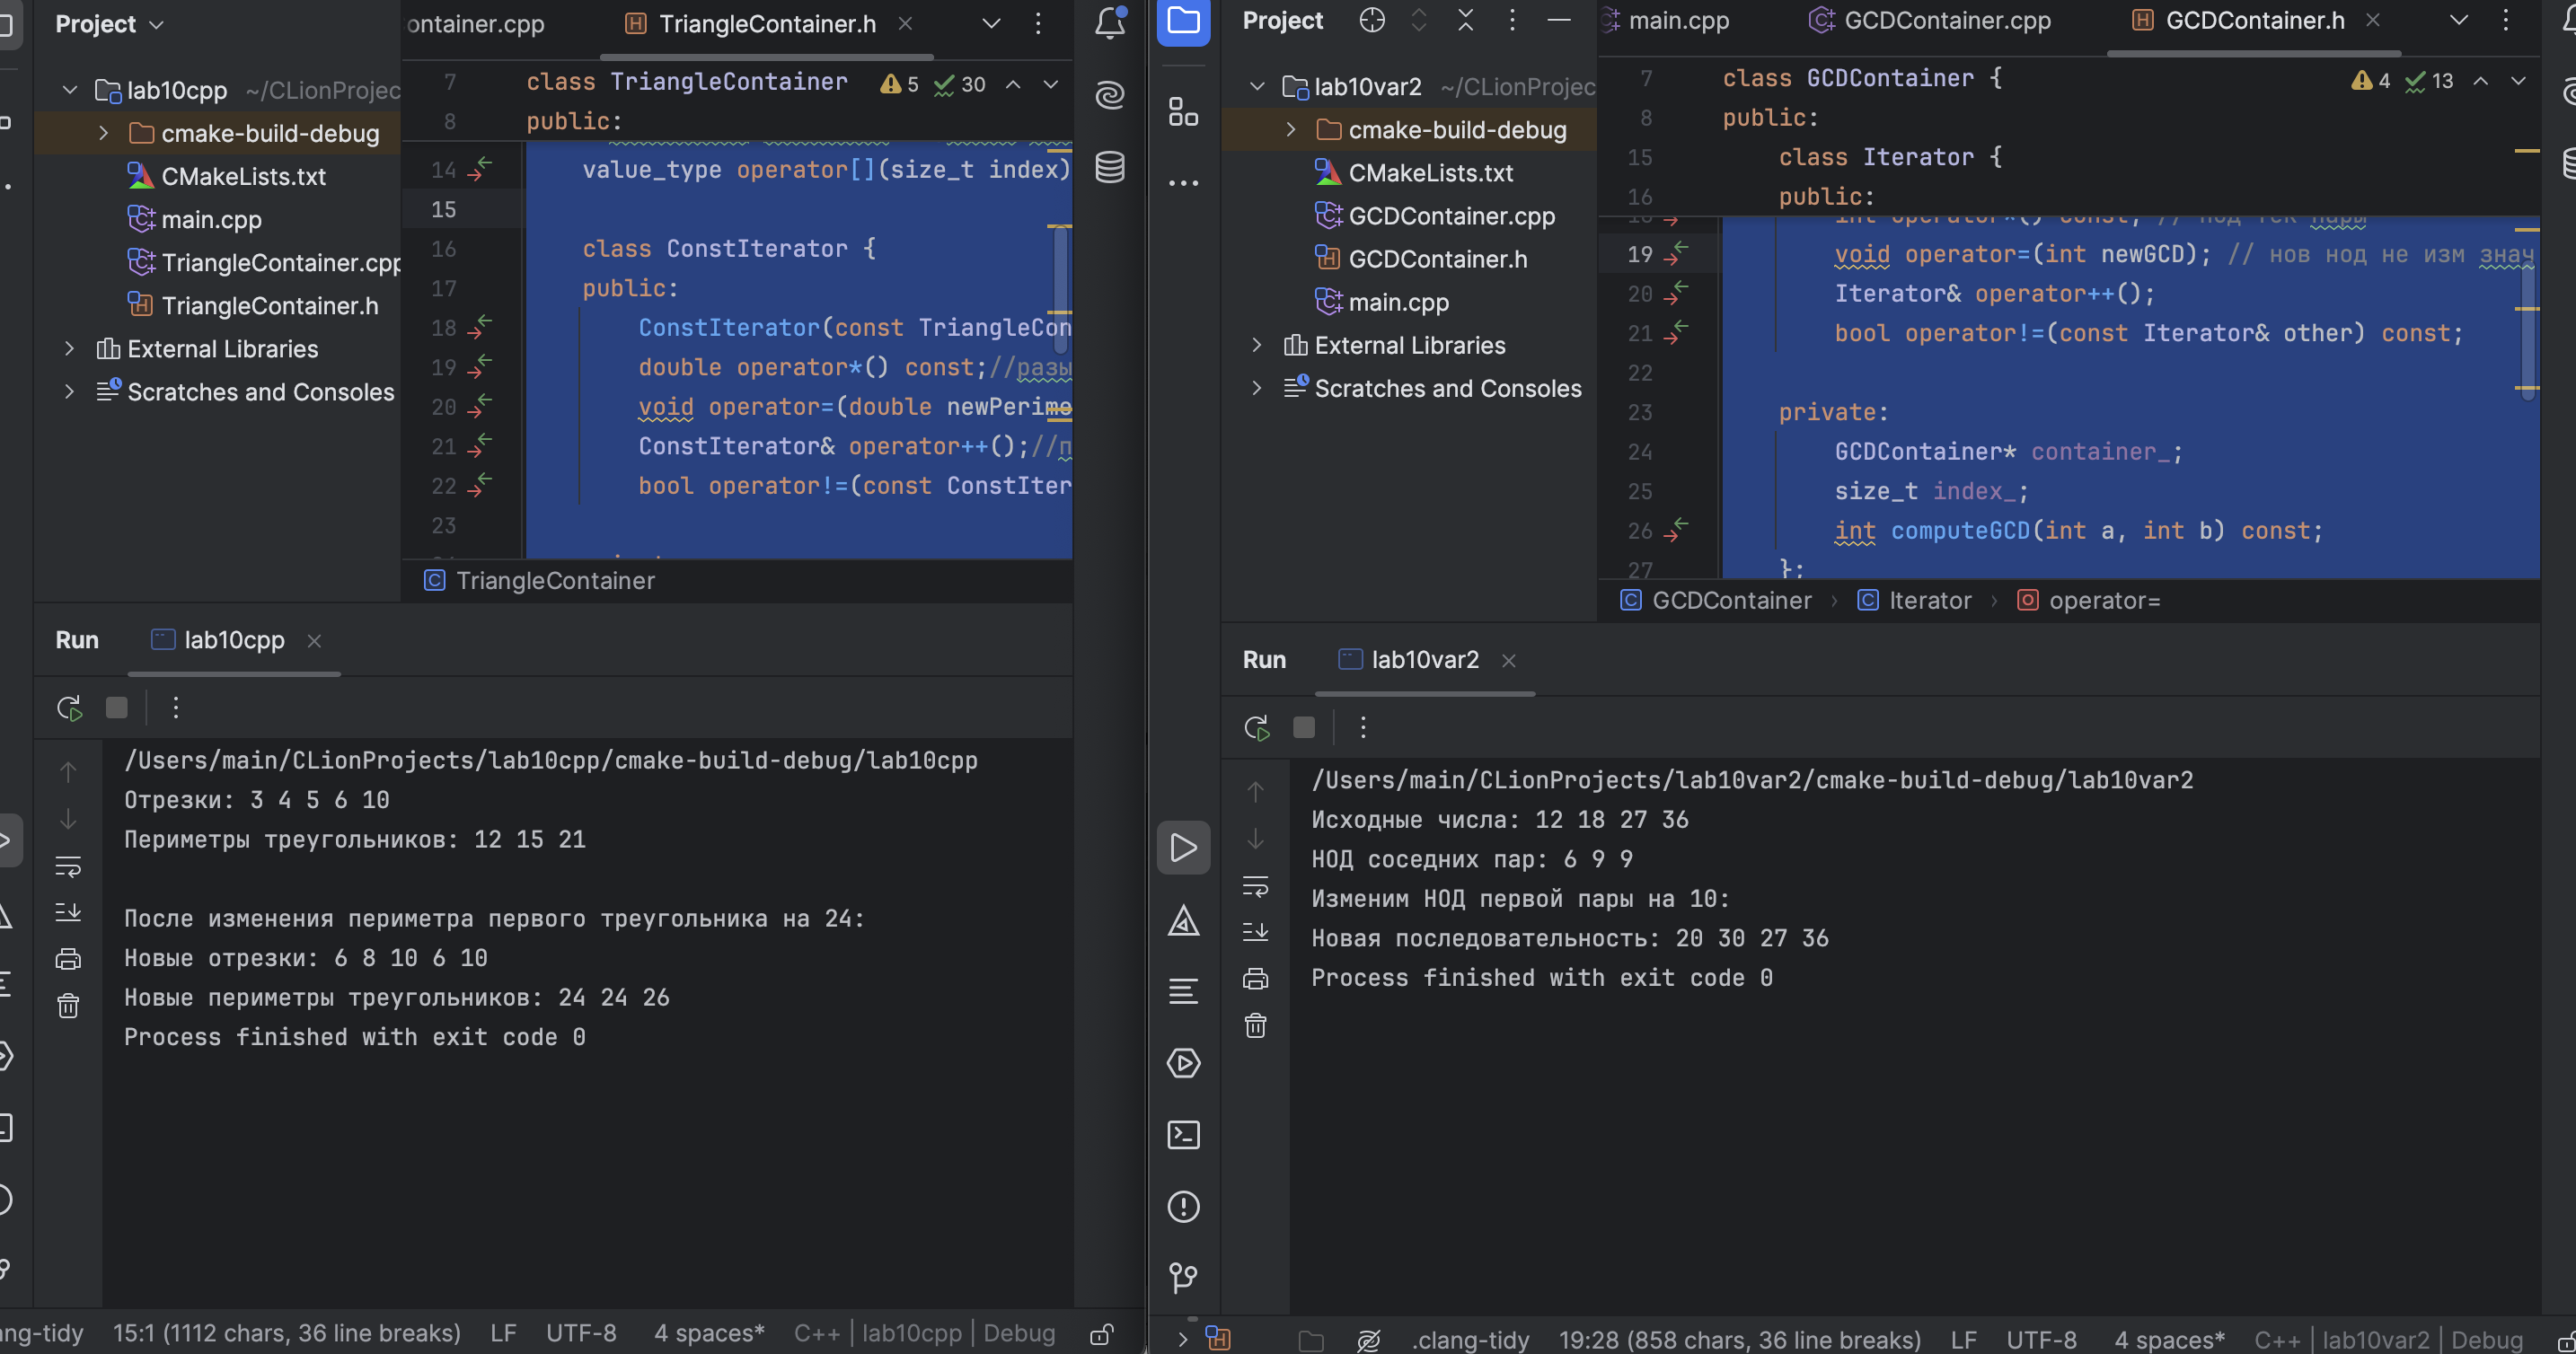
\includegraphics[width=0.8\textwidth]{фото23.jpeg}
  \captionof{figure}{Фрагменты вывода тестовых программ}
\end{center}

%--------------------------------------
\section{Вывод}
В ходе лабораторной работы были разработаны два контейнерных класса с
нестандартными \emph{итераторами}:

\begin{itemize}[nosep]
  \item \textbf{GCDContainer} — последовательность целых с итератором,
        перебирающим НО Д соседних чисел и позволяющим
        \emph{массово} менять их общий делитель;
  \item \textbf{TriangleContainer} — последовательность отрезков с
        \emph{константным} итератором по периметрам треугольников,
        образованных тремя соседними отрезками, с поддержкой
        масштабирования без изменения углов.
\end{itemize}

Обе структуры предоставляют привычный синтаксис
доступа~\lstinline|[ ]|, корректно обрабатывают граничные ситуации и
демонстрируют принципы проектирования собственных итераторов в C++.
\end{document}
